\chapter{Perancangan}
\label{chap:perancangan}
Untuk mempropagasi email, diperlukan perancangan sistem dan beberapa peran yang harus dilakukan oleh partisipan. 

\section{\textit{Event} yang Terkait dengan Integrasi Sistem Email}
\label{sec:eventUserTask}

Integrasi Camunda dengan sistem email pada skripsi ini bertujuan untuk memberi tahu aktor Camunda apabila ada \textit{tasks} yang perlu dikerjakan oleh aktor. Ketika aktor menerima email mengenai \textit{tasks} yang perlu dikejakan, aktor dapat langsung mengerjakannya. 

Camunda memiliki berbagai jenis \textit{tasks} seperti \textit{user tasks, manual tasks, service task}, dan lainnya. Karena proses integrasi email dengan Camunda melibatkan aktor (aktor menerima pemberitahuan pekerjaannya melalui email), \textit{task} yang akan diintegrasikan dengan sistem email adalah \textit{user tasks}.

\section{Mekanisme Integrasi Sistem Email}
\label{integrasi}
\textit{User tasks} memiliki atribut \textit{Task Listener} yang dapat mengeksekusi perintah. \textit{Task Listener} memiliki dua atribut, yaitu \textit{Event Type} dan \textit{Listener Type}. Terdapat empat pilihan dari \textit{Event Type}, yaitu \textit{create, assignment, complete, delete}. 
		\begin{figure}[H]
			\centering
			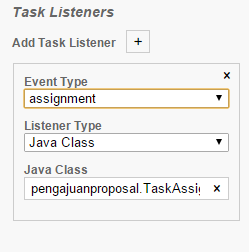
\includegraphics[scale=1]{Gambar/Bab-3/TaskListener}
			\caption{Event Task Listener} 
			\label{fig:eventtasklistener}
		\end{figure}
\begin{itemize}
	\item Create, perintah dieksekusi ketika \textit{task} telah dibuat dan siap untuk dikerjakan. 
	\item Assignment, perintah dieksekusi ketika aktor yang akan mengerjakan \textit{task} sudah ditentukan.
	\item Complete, perintah dieksekusi ketika \textit{task} sudah dikerjakan dan sebelum \textit{task} dihapus.
	\item Delete, perintah dieksekusi setelah \textit{task} dihapus.
\end{itemize}


Untuk mengintegrasikan \textit{user tasks} dengan email, \textit{event type} yang dapat digunakan adalah \textit{create} dan \textit{assignment}. \textit{Event complete} dan \textit{delete} tidak dapat digunakan untuk memberi tahu aktor karena setelah \textit{task} selesai dan dihapus, alamat email untuk \textit{Task} selanjutnya belum diambil sementara \textit{event} sudah selesai dipanggil.

Apabila menggunakan \textit{event create}, \textit{task} harus memiliki pemiliknya masing-masing ketika BPMN dibuat atau memiliki \textit{candidate user/group}. Bila pemilik \textit{task} belum ditentukan, email tidak akan terkirim, karena \textit{event create} sudah selesai dipanggil sebelum \textit{task} memiliki pemilik. Pengiriman email untuk \textit{task} yang belum memiliki aktor dapat menggunakan \textit{event create}. Sedangkan pada \textit{event assignment}, pengiriman email dilakukan setelah \textit{task} didelegasikan ke masing-masing user.





\section{Perancangan Sistem}
\label{rancangansistem}
Berdasarkan analisis di bab sebelumnya, maka untuk mempropagasi email diperlukan beberapa persyaratan, yaitu :
\begin{enumerate}
	\item Model proses menggunakan BPMN yang sudah dilengkapi form HTML untuk \textit{user task}, implementasi untuk \textit{service task} dan atribut lain yang diperlukan.
	\item Kumpulan \textit{user/group} yang akan mengerjakan tugas.
	\item Alamat email yang merepresentasikan sistem.
	\item Algoritma untuk mengirim email.
	\item Business Process Management System (BPMS), yaitu tools untuk mengotomasi jalannya proses.
\end{enumerate}

\subsection{Email}
\label{email}
Alamat email yang digunakan untuk merepresentasikan sistem berbasis Gmail SMTP. Gmail SMTP yang akan digunakan memiliki konfigurasi sebagai berikut \cite{smtpgoogle} :
\begin{itemize}
	\item Alamat server = smtp.gmail.com.
	\item Port = 587.
	\item Username Gmail.
	\item Password Gmail.
\end{itemize}
Email yang akan dikirimkan ke aktor memiliki format :
\begin{enumerate}
	\item Subjek :
	\item Nama aktor.
	\item Nama \textit{task}.
	\item Link ke \textit{task}, yaitu http://localhost/camunda/app/tasklist/default/\#/?task=(\textit{id task}).
\end{enumerate} 

\subsection{Algoritma Pengiriman Email}
\label{sec:algoritma}

Berikut adalah algoritma untuk mengirimkan email.
\begin{enumerate}
	\item Mengambil id dari \textit{task}.
	\item Mengambil email aktor yang akan mengerjakan \textit{task}.
	\item Membangkitkan subjek dan isi email yang berisi tautan ke task yang akan dikerjakan. Tautan didapatkan dari id \textit{task}.
	\item Membuat koneksi ke email server dengan \textit{username} dan \textit{password}
	\item Mengirim email.
\end{enumerate}


\section{Peran Partisipan}
\label{peranpartisipan}
Setiap partisipan memiliki perannya masing-masing. Desainer bertugas merancang BPMN, admin bertugas mengatur jalannya otomasi proses bisnis, sedangkan aktor bertugas mengerjakan \textit{tasks}
\subsection{Tugas Desainer}
\label{tugasdesainer}
Berdasarkan perancangan sistem di atas, seorang desainer model proses memiliki beberapa tugas, yaitu :
\begin{enumerate}
	\item Merancang model proses.
	\item Menambahkan form HTML pada \textit{user task}, \textit{implementasi service task}, \textit{task listener} untuk propagasi email, dan berbagai atribut lainnnya sesuai kebutuhan.
	\item Mendelegasikan task kepada user/group yang akan mengerjakan.
\end{enumerate}

\subsection{Tugas Admin}	
\label{tugasadmin}
\begin{enumerate}
	\item Membuat alamat email yang merepresentasikan sistem.
	\item Menambahkan \textit{username}, \textit{password}, dan \textit{host} email pada kode task listener yang berhubungan dengan propagasi email.
	\item Menambahkan user/group yang akan mengerjakan \textit{tasks} pada Camunda Admin.
	\item Menjalankan dan memulai proses.
\end{enumerate}

\subsection{Tugas Aktor}
\label{tugasaktor}
	\begin{enumerate}
	\item Memberitahu alamat email kepada admin.
	\item Mengerjakan \textit{task}.
\end{enumerate}


\subsection{Perancangan Aktor}
\label{perancanganaktor}
Untuk pengujian skenario, ada beberapa aktor yang dibuat, yaitu :
\begin{enumerate}
	\item John, dengan alamat email johncamunda@gmail.com dan bagian dari grup \textit{sales}.
	\item Mary, dengan alamat email marycamunda@gmail.com dan bagian dari grup \textit{accounting}.
	\item Peter, dengan alamat email petercamunda@gmail.com dan bagian dari grup \textit{management}.
\end{enumerate}